\section{Vector Autoregressive Model}
\label{sec:VAR}
The Vector Autoregressive (VAR) model extends the single-variable Autoregressive (AR) model discussed in Section \ref{sec:AR} to accommodate multiple time series. VAR models enable the analysis of dynamic relationships between interacting variables by allowing for feedback among them, making these models useful also for forecasting purposes. \\
Formally, a VAR model of order $p$ (VAR($p$)) for $K$ variables is represented as:
\begin{equation}
    \mathbf{y}_t = \bm{\mu}_0 + A_1 \mathbf{y}_{t-1} + A_2 \mathbf{y}_{t-2} + \cdots + A_p \mathbf{y}_{t-p} + \bm{\epsilon}_t
\end{equation}
where:
\begin{itemize}
    \item $p$ is the number of past time periods considered.
    \item $\bm{\mu}_0$ is a $K \times 1$ vector of constants.
    \item $\mathbf{y}_t$ is a $K \times 1$ vector of variables at time $t$.
    \item $A_i$ (for $i = 1, 2, \ldots, p$) are $K \times K$ coefficient matrices.
    \item $\bm{\epsilon}_t$ is a $K \times 1$ vector of error terms at time $t$.
\end{itemize}
For our analysis, we implement a VAR model of order 1 (VAR(1)).
\subsection*{VAR(1)}
The VAR(1) model for $K = 2$ is defined as:
\begin{equation}
    \label{eq:VAR1}
    \begin{pmatrix}
        \ \ \ y_{1,t} \\
        \ \ \ y_{2,t}
    \end{pmatrix}
    =
    \begin{pmatrix}
        \ \ \ \mu_{0,1} \\
        \ \ \ \mu_{0,2}
    \end{pmatrix}
    +
    \begin{pmatrix}
        \ \ \ a_{11} & a_{12} \\
        \ \ \ a_{21} & a_{22}
    \end{pmatrix}
    \begin{pmatrix}
        \ \ \ y_{1, t-1} \\
        \ \ \ y_{2, t-1}
    \end{pmatrix}
    +
    \begin{pmatrix}
        \ \ \ \epsilon_{1,t} \\
        \ \ \ \epsilon_{2,t}
    \end{pmatrix}
\end{equation}
or more compactly:
\begin{equation}
    \label{eq:VAR1_compact}
    \mathbf{y}_t = \bm{\mu}_0 + A \mathbf{y}_{t-1} + \bm{\epsilon}_t
\end{equation}
Here, \(y_{1,t}\) represents the GDP\_PC1 variable and \(y_{2,t}\) represents the CPIAUCSL\_PC1 variable at time $t$. \\
Assuming that $\bm{\epsilon}_t$ follows a multivariate normal distribution with $\bm{0}$ mean and covariance matrix $\Sigma$, the likelihood is:
\begin{equation}
    \label{eq:VAR1_likelihood}
    \mathbf{y}_{t}|\bm{\mu}_{0}, A, \Sigma, \mathbf{y}_{t-1} \sim \mathcal{N}_2(\bm{\mu}_{0} + A \mathbf{y}_{t-1}, \Sigma)
\end{equation}
For the priors, we chose:
\begin{equation}
    \label{eq:VAR1_priors}
    \begin{split}
        \mu_{0,i} \sim \mathcal{N}(0.0, 10000) \quad \quad i = 1, 2\\
        a_{ij} \sim \mathcal{U}(-1, 1) \quad \quad i,j = 1, 2 \\
        \Omega = \Sigma^{-1} \sim Wishart(R, 3)
    \end{split}
\end{equation}
where: 
\begin{equation}
    R = 
    \begin{pmatrix}
        \ \ \ 1 & 0.5 \\
        \ \ \ 0.5 & 1
    \end{pmatrix}
\end{equation}
The priors are chosen to be uninformative. \\
Using JAGS to implement the VAR(1) model for GDP and CPIAUCSL, we obtained the posterior distributions shown in Figure \ref{fig:VAR1_posteriors}, with the corresponding means and 95\% credible intervals reported in Table \ref{tab:VAR1_posteriors}. \\
\begin{figure}[H]
    \centering
    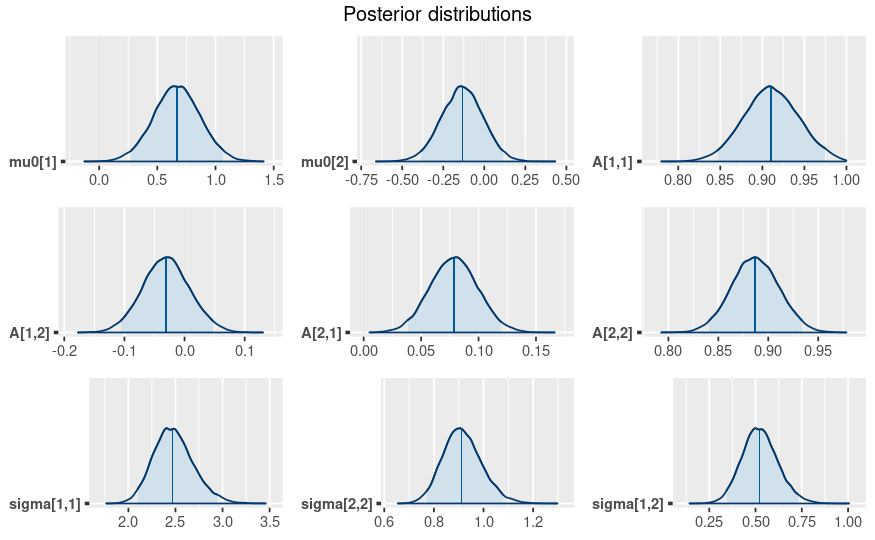
\includegraphics[width=0.8\textwidth]{images/6-VAR/posteriors.png}
    \caption{Posterior distributions of the parameters for the VAR(1) model.}
    \label{fig:VAR1_posteriors}
\end{figure}
\begin{table}[H]
    \centering
    \begin{tabular}{c|c|c}
        \textbf{Parameter } & \textbf{Posterior Mean } & \textbf{95\% Credible Interval } \\
        \cline{1-3}
        $\mu_{0,1}$     &  0.66929256 &  (0.27516565, 1.06102229) \\
        $\mu_{0,2}$     & -0.13454152 &  (-0.38389818, 0.11090167) \\
        $a_{11}$     &  0.91055747 &  (0.84673870, 0.97466996) \\
        $a_{12}$     & -0.03039508 &  (-0.10650041, 0.04742719) \\
        $a_{21}$     &  0.07867888 &  (0.03824313, 0.11987435) \\
        $a_{22}$     &  0.88708627 &  (0.84108698, 0.93353337) \\
        $\Sigma_{11}$ &  2.48031746 &  (2.09784974, 2.94229950) \\
        $\Sigma_{12}$ &  0.52456983 &  (0.34405208, 0.72777246) \\
        $\Sigma_{22}$ &  0.91495776 &  (0.77210667, 1.07984048) \\
    \end{tabular}
    \caption{Posterior means and 95\% credible intervals for the parameters of the VAR(1) model.}
    \label{tab:VAR1_posteriors}
\end{table}
Lastly, we plotted the in-sample and out-of-sample predictions with 95\% credible intervals and compared them with the actual data. The results are shown in Figures \ref{fig:VAR1_gdp_prediction} and \ref{fig:VAR1_infl_prediction}. \\ 
Analyzing the out-of-sample predictions, we observe that in the VAR(1) model, GDP values impact CPIAUCSL, resulting in slightly different predictions compared to the AR(1) model for CPIAUCSL.
\begin{figure}[H]
    \centering
    \begin{minipage}{0.5\textwidth}
        \centering
        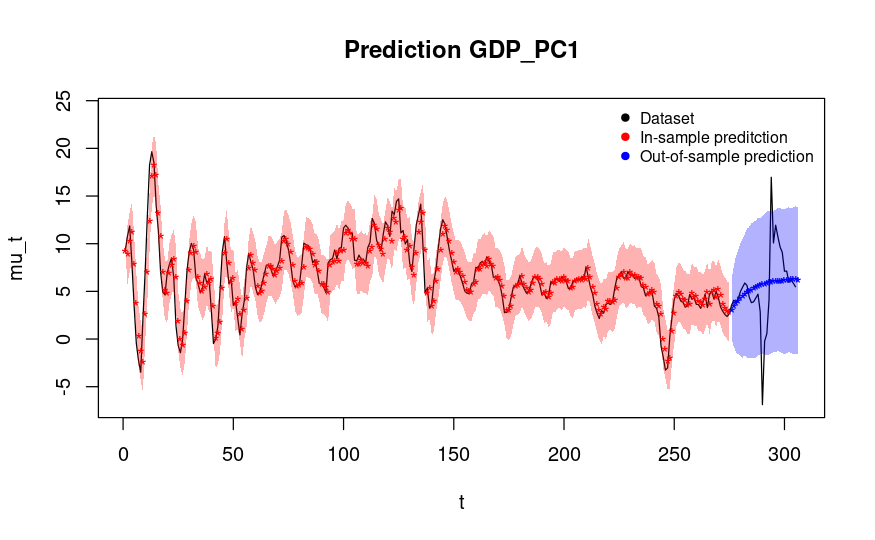
\includegraphics[width=\textwidth]{images/6-VAR/gdp_prediction.png}
        \caption{In-sample and out-of-sample predictions for the GDP using the VAR(1) model.}
        \label{fig:VAR1_gdp_prediction} 
    \end{minipage}\hfill
    \begin{minipage}{0.5\textwidth}
        \centering
        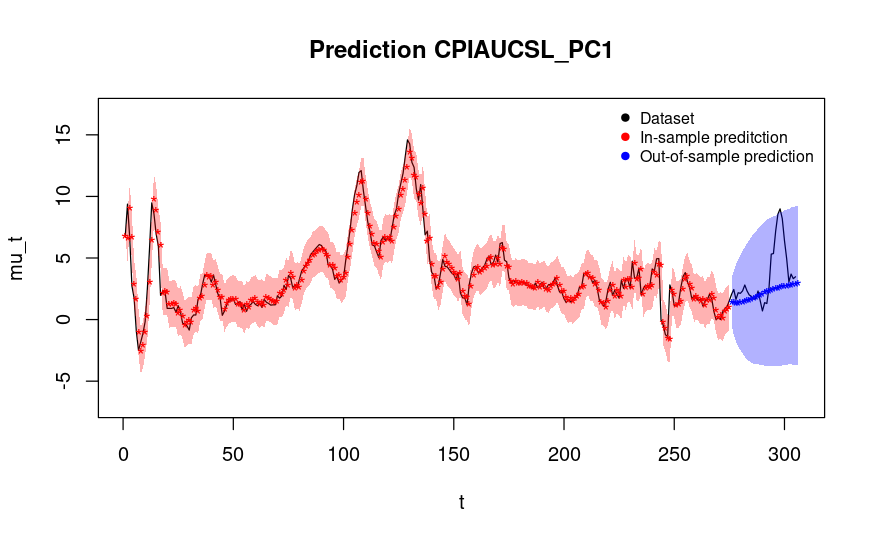
\includegraphics[width=\textwidth]{images/6-VAR/infl_prediction.png}
        \caption{In-sample and out-of-sample predictions for the CPIAUCSL using the VAR(1) model.}
        \label{fig:VAR1_infl_prediction}
    \end{minipage}
\end{figure}
Lastly, we compared our results with those obtained using the VAR function in R. This comparison revealed no significant differences between the two sets of results.